% Options for packages loaded elsewhere
\PassOptionsToPackage{unicode}{hyperref}
\PassOptionsToPackage{hyphens}{url}
\documentclass[
]{article}
\usepackage{xcolor}
\usepackage[margin=1in]{geometry}
\usepackage{amsmath,amssymb}
\setcounter{secnumdepth}{-\maxdimen} % remove section numbering
\usepackage{iftex}
\ifPDFTeX
  \usepackage[T1]{fontenc}
  \usepackage[utf8]{inputenc}
  \usepackage{textcomp} % provide euro and other symbols
\else % if luatex or xetex
  \usepackage{unicode-math} % this also loads fontspec
  \defaultfontfeatures{Scale=MatchLowercase}
  \defaultfontfeatures[\rmfamily]{Ligatures=TeX,Scale=1}
\fi
\usepackage{lmodern}
\ifPDFTeX\else
  % xetex/luatex font selection
\fi
% Use upquote if available, for straight quotes in verbatim environments
\IfFileExists{upquote.sty}{\usepackage{upquote}}{}
\IfFileExists{microtype.sty}{% use microtype if available
  \usepackage[]{microtype}
  \UseMicrotypeSet[protrusion]{basicmath} % disable protrusion for tt fonts
}{}
\makeatletter
\@ifundefined{KOMAClassName}{% if non-KOMA class
  \IfFileExists{parskip.sty}{%
    \usepackage{parskip}
  }{% else
    \setlength{\parindent}{0pt}
    \setlength{\parskip}{6pt plus 2pt minus 1pt}}
}{% if KOMA class
  \KOMAoptions{parskip=half}}
\makeatother
\usepackage{color}
\usepackage{fancyvrb}
\newcommand{\VerbBar}{|}
\newcommand{\VERB}{\Verb[commandchars=\\\{\}]}
\DefineVerbatimEnvironment{Highlighting}{Verbatim}{commandchars=\\\{\}}
% Add ',fontsize=\small' for more characters per line
\usepackage{framed}
\definecolor{shadecolor}{RGB}{248,248,248}
\newenvironment{Shaded}{\begin{snugshade}}{\end{snugshade}}
\newcommand{\AlertTok}[1]{\textcolor[rgb]{0.94,0.16,0.16}{#1}}
\newcommand{\AnnotationTok}[1]{\textcolor[rgb]{0.56,0.35,0.01}{\textbf{\textit{#1}}}}
\newcommand{\AttributeTok}[1]{\textcolor[rgb]{0.13,0.29,0.53}{#1}}
\newcommand{\BaseNTok}[1]{\textcolor[rgb]{0.00,0.00,0.81}{#1}}
\newcommand{\BuiltInTok}[1]{#1}
\newcommand{\CharTok}[1]{\textcolor[rgb]{0.31,0.60,0.02}{#1}}
\newcommand{\CommentTok}[1]{\textcolor[rgb]{0.56,0.35,0.01}{\textit{#1}}}
\newcommand{\CommentVarTok}[1]{\textcolor[rgb]{0.56,0.35,0.01}{\textbf{\textit{#1}}}}
\newcommand{\ConstantTok}[1]{\textcolor[rgb]{0.56,0.35,0.01}{#1}}
\newcommand{\ControlFlowTok}[1]{\textcolor[rgb]{0.13,0.29,0.53}{\textbf{#1}}}
\newcommand{\DataTypeTok}[1]{\textcolor[rgb]{0.13,0.29,0.53}{#1}}
\newcommand{\DecValTok}[1]{\textcolor[rgb]{0.00,0.00,0.81}{#1}}
\newcommand{\DocumentationTok}[1]{\textcolor[rgb]{0.56,0.35,0.01}{\textbf{\textit{#1}}}}
\newcommand{\ErrorTok}[1]{\textcolor[rgb]{0.64,0.00,0.00}{\textbf{#1}}}
\newcommand{\ExtensionTok}[1]{#1}
\newcommand{\FloatTok}[1]{\textcolor[rgb]{0.00,0.00,0.81}{#1}}
\newcommand{\FunctionTok}[1]{\textcolor[rgb]{0.13,0.29,0.53}{\textbf{#1}}}
\newcommand{\ImportTok}[1]{#1}
\newcommand{\InformationTok}[1]{\textcolor[rgb]{0.56,0.35,0.01}{\textbf{\textit{#1}}}}
\newcommand{\KeywordTok}[1]{\textcolor[rgb]{0.13,0.29,0.53}{\textbf{#1}}}
\newcommand{\NormalTok}[1]{#1}
\newcommand{\OperatorTok}[1]{\textcolor[rgb]{0.81,0.36,0.00}{\textbf{#1}}}
\newcommand{\OtherTok}[1]{\textcolor[rgb]{0.56,0.35,0.01}{#1}}
\newcommand{\PreprocessorTok}[1]{\textcolor[rgb]{0.56,0.35,0.01}{\textit{#1}}}
\newcommand{\RegionMarkerTok}[1]{#1}
\newcommand{\SpecialCharTok}[1]{\textcolor[rgb]{0.81,0.36,0.00}{\textbf{#1}}}
\newcommand{\SpecialStringTok}[1]{\textcolor[rgb]{0.31,0.60,0.02}{#1}}
\newcommand{\StringTok}[1]{\textcolor[rgb]{0.31,0.60,0.02}{#1}}
\newcommand{\VariableTok}[1]{\textcolor[rgb]{0.00,0.00,0.00}{#1}}
\newcommand{\VerbatimStringTok}[1]{\textcolor[rgb]{0.31,0.60,0.02}{#1}}
\newcommand{\WarningTok}[1]{\textcolor[rgb]{0.56,0.35,0.01}{\textbf{\textit{#1}}}}
\usepackage{graphicx}
\makeatletter
\newsavebox\pandoc@box
\newcommand*\pandocbounded[1]{% scales image to fit in text height/width
  \sbox\pandoc@box{#1}%
  \Gscale@div\@tempa{\textheight}{\dimexpr\ht\pandoc@box+\dp\pandoc@box\relax}%
  \Gscale@div\@tempb{\linewidth}{\wd\pandoc@box}%
  \ifdim\@tempb\p@<\@tempa\p@\let\@tempa\@tempb\fi% select the smaller of both
  \ifdim\@tempa\p@<\p@\scalebox{\@tempa}{\usebox\pandoc@box}%
  \else\usebox{\pandoc@box}%
  \fi%
}
% Set default figure placement to htbp
\def\fps@figure{htbp}
\makeatother
\setlength{\emergencystretch}{3em} % prevent overfull lines
\providecommand{\tightlist}{%
  \setlength{\itemsep}{0pt}\setlength{\parskip}{0pt}}
\usepackage{bookmark}
\IfFileExists{xurl.sty}{\usepackage{xurl}}{} % add URL line breaks if available
\urlstyle{same}
\hypersetup{
  pdftitle={Simulation Results},
  hidelinks,
  pdfcreator={LaTeX via pandoc}}

\title{Simulation Results}
\author{}
\date{\vspace{-2.5em}}

\begin{document}
\maketitle

\begin{Shaded}
\begin{Highlighting}[]
\FunctionTok{source}\NormalTok{(}\StringTok{"process{-}simulation{-}results.R"}\NormalTok{)}
\end{Highlighting}
\end{Shaded}

\begin{verbatim}
## -- Attaching core tidyverse packages ------------------------ tidyverse 2.0.0 --
## v dplyr     1.1.4     v readr     2.1.5
## v forcats   1.0.0     v stringr   1.5.1
## v ggplot2   3.5.2     v tibble    3.2.1
## v lubridate 1.9.3     v tidyr     1.3.1
## v purrr     1.0.4     
## -- Conflicts ------------------------------------------ tidyverse_conflicts() --
## x dplyr::filter() masks stats::filter()
## x dplyr::lag()    masks stats::lag()
## i Use the conflicted package (<http://conflicted.r-lib.org/>) to force all conflicts to become errors
\end{verbatim}

\begin{Shaded}
\begin{Highlighting}[]
\NormalTok{CML\_bias }\OtherTok{\textless{}{-}} 
\NormalTok{  mu\_graph\_res }\SpecialCharTok{\%\textgreater{}\%}
  \FunctionTok{filter}\NormalTok{(estimator }\SpecialCharTok{==} \StringTok{"CML"}\NormalTok{) }\SpecialCharTok{\%\textgreater{}\%}
  \FunctionTok{summarize}\NormalTok{(}
    \AttributeTok{max\_abs\_bias =} \FunctionTok{max}\NormalTok{(}\FunctionTok{abs}\NormalTok{(bias))}
\NormalTok{  )}

\NormalTok{convergence\_min }\OtherTok{\textless{}{-}} 
\NormalTok{  mu\_graph\_res }\SpecialCharTok{\%\textgreater{}\%}
  \FunctionTok{filter}\NormalTok{(model }\SpecialCharTok{==} \StringTok{"3PSM"}\NormalTok{) }\SpecialCharTok{\%\textgreater{}\%}
  \FunctionTok{group\_by}\NormalTok{(estimator) }\SpecialCharTok{\%\textgreater{}\%}
  \FunctionTok{filter}\NormalTok{(}
\NormalTok{    convergence }\SpecialCharTok{==} \FunctionTok{min}\NormalTok{(convergence)}
\NormalTok{  )}
\end{Highlighting}
\end{Shaded}

We organize our presentation of simulation study results by first
considering the properties of point and interval estimators for the
average effect size. For this parameter, we compare the bias and
accuracy of the CML and ARGL estimators to that of the CHE-ISCW
estimator and the PET/PEESE estimator. We also examine the calibration
of cluster-robust and bootstrap confidence intervals based on the CML
and ARGL estimators. We then briefly consider the bias and accuracy of
estimators of the marginal variance of the effect size distribution and
the selection parameter in the step-function model.

\subsection{Average Effect Size}\label{average-effect-size}

The CHE-ISCW and PET/PEESE estimators produced results for every
replication in every condition. The CML and ARGL estimators for the
step-function selection model had very high convergence rates across
most conditions, although the CML estimator did exhibit rates of
convergence below 99\% under conditions with the lowest degree of
heterogeneity \(\tau = 0.05\), with the lowest convergence rate of
94.4\%. For the ARGL estimator, convergence was above 99.8\% across all
conditions. Supplementary Figure @ref(fig:convergence-rates) depicts the
range of convergence rates of the CML and ARGL estimators. We evaluated
the performance characteristics of these estimators across replications
where they converged.

\subsubsection{Bias}\label{bias}

\begin{Shaded}
\begin{Highlighting}[]
\FunctionTok{ggplot}\NormalTok{(mu\_graph\_res) }\SpecialCharTok{+} 
  \FunctionTok{aes}\NormalTok{(}\AttributeTok{x =}\NormalTok{ weights, }\AttributeTok{y =}\NormalTok{ bias, }\AttributeTok{color =}\NormalTok{ estimator, }\AttributeTok{fill =}\NormalTok{ estimator) }\SpecialCharTok{+}
  \FunctionTok{geom\_hline}\NormalTok{(}\AttributeTok{yintercept =} \DecValTok{0}\NormalTok{) }\SpecialCharTok{+}
  \FunctionTok{geom\_boxplot}\NormalTok{(}\AttributeTok{alpha =}\NormalTok{ .}\DecValTok{5}\NormalTok{, }\AttributeTok{coef =} \ConstantTok{Inf}\NormalTok{) }\SpecialCharTok{+}
  \FunctionTok{scale\_color\_brewer}\NormalTok{(}\AttributeTok{palette =} \StringTok{"Dark2"}\NormalTok{) }\SpecialCharTok{+}
  \FunctionTok{scale\_fill\_brewer}\NormalTok{(}\AttributeTok{palette =} \StringTok{"Dark2"}\NormalTok{) }\SpecialCharTok{+}
  \FunctionTok{scale\_x\_discrete}\NormalTok{(}\AttributeTok{labels =} \ControlFlowTok{function}\NormalTok{(x) stringr}\SpecialCharTok{::}\FunctionTok{str\_wrap}\NormalTok{(x, }\AttributeTok{width =} \DecValTok{3}\NormalTok{))}\SpecialCharTok{+}
  \FunctionTok{facet\_grid}\NormalTok{(}
\NormalTok{    tau }\SpecialCharTok{\textasciitilde{}}\NormalTok{ mean\_smd, }
    \AttributeTok{labeller =} \FunctionTok{label\_bquote}\NormalTok{(}
      \AttributeTok{rows =}\NormalTok{ tau }\SpecialCharTok{==}\NormalTok{ .(tau),}
      \AttributeTok{cols =}\NormalTok{ mu }\SpecialCharTok{==}\NormalTok{ .(mean\_smd)}
\NormalTok{    ),}
    \AttributeTok{scales =} \StringTok{"free\_y"}
\NormalTok{  ) }\SpecialCharTok{+}
  \FunctionTok{labs}\NormalTok{(}
    \AttributeTok{x =} \StringTok{"Selection probability"}\NormalTok{, }
    \AttributeTok{y =} \StringTok{"Bias"}\NormalTok{, }
    \AttributeTok{color =} \StringTok{"Estimator"}\NormalTok{,}
    \AttributeTok{fill =} \StringTok{"Estimator"}
\NormalTok{  ) }\SpecialCharTok{+} 
  \FunctionTok{theme\_bw}\NormalTok{() }\SpecialCharTok{+}
  \FunctionTok{theme}\NormalTok{(}\AttributeTok{legend.position =} \StringTok{"top"}\NormalTok{)}
\end{Highlighting}
\end{Shaded}

\begin{sidewaysfigure}
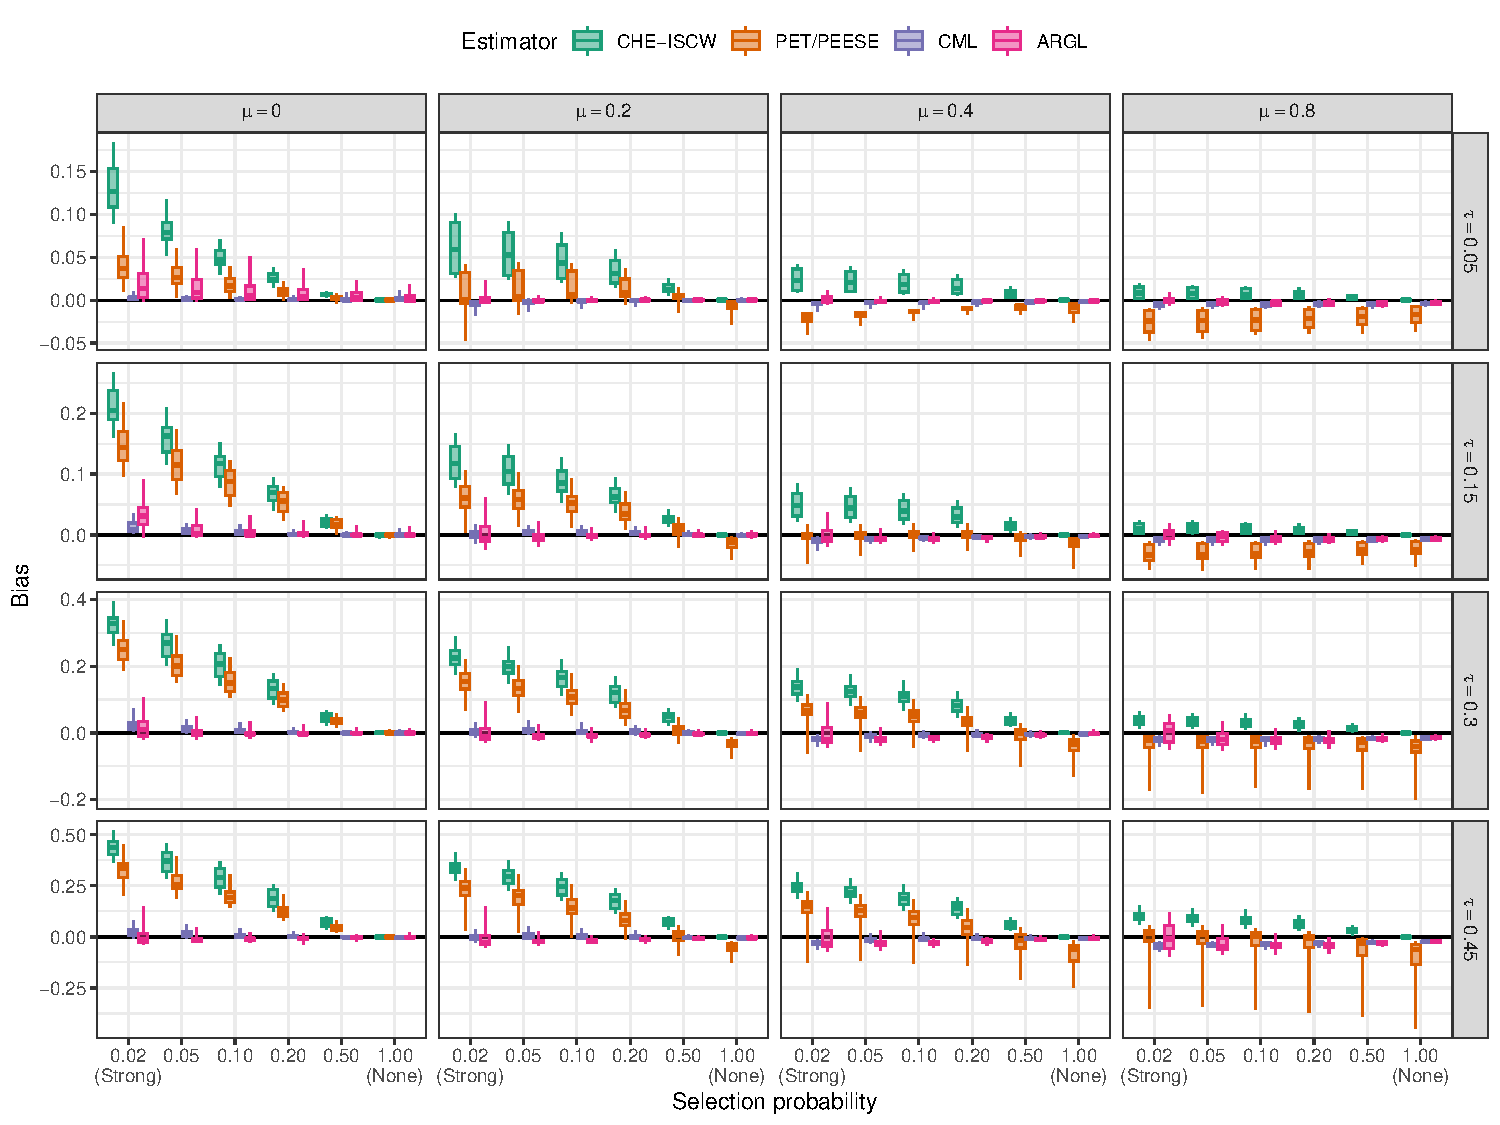
\includegraphics{simulation_results_files/figure-latex/mu-bias-1} \caption{Bias for estimators of average effect size by selection probability, average SMD, and between-study heterogeneity}\label{fig:mu-bias}
\end{sidewaysfigure}

Figure @ref(fig:mu-bias) depicts the bias (represented on the vertical
axis of each plot) of each estimator of average effect size as a
function of the strength of selective reporting (represented on the
horizontal axis of each plot), average effect size parameter (varying by
grid column), and between-study heterogeneity (\(\tau\), varying by grid
row). The box plot for each estimator depicts variation in bias over the
remaining factors in the simulation design. Note that the range of the
vertical axis differs by grid row because the bias of some estimators is
strongly influenced by the degree of heterogeneity.

The CML estimator has negligible or small bias across all conditions.
Its largest bias was 0.08, occurring when selective reporting is very
strong, average effect size is zero, and heterogeneity is large. The
small bias of the CML estimator is stable across varying degrees of
outcome correlation, within-study heterogeneity, number of observed
studies, and primary study sample size. Similar to the CML estimator,
the ARGL estimator also has negligible or small bias across most
conditions, although it becomes more biased when average effect is zero
and selection is very strong.

In contrast to the estimators based on the marginal selection model, the
comparison estimators are systematically biased under many conditions.
The CHE-ISCW estimator, which does not directly adjust for selective
reporting, is systematically biased under conditions with non-null
selection. When average effect size is large \((\mu = 0.8)\), its bias
remains quite small even when selective reporting is very strong.
However, the bias of CHE-ISCW grows stronger when selection is more
extreme, when average effect size is smaller, and when heterogeneity is
larger, exceeding 0.50 when \(\mu = 0.0\), \(\tau = 0.45\), and
\(\lambda_1 = 0.02\). Although the PET/PEESE estimator uses a regression
adjustment to account for possible selective reporting, it too becomes
severely biased when selective reporting is strong. For smaller values
of average effect size \((\mu \leq 0.2)\), the bias of PET/PEESE tracks
the bias of the CHE-ISCW estimator but is somewhat less pronounced; its
bias grows stronger for smaller values of average effect size and higher
levels of heterogeneity. For larger values of average effect size
\((\mu = 0.8)\), the PET/PEESE estimator is negatively biased,
systematically under-estimating the average effect size---especially at
high levels of heterogeneity.

\subsubsection{Scaled RMSE}\label{scaled-rmse}

\begin{Shaded}
\begin{Highlighting}[]
\FunctionTok{ggplot}\NormalTok{(mu\_graph\_res) }\SpecialCharTok{+} 
  \FunctionTok{aes}\NormalTok{(}\AttributeTok{x =}\NormalTok{ weights, }\AttributeTok{y =}\NormalTok{ scrmse, }\AttributeTok{color =}\NormalTok{ estimator, }\AttributeTok{fill =}\NormalTok{ estimator) }\SpecialCharTok{+}
  \FunctionTok{geom\_hline}\NormalTok{(}\AttributeTok{yintercept =} \DecValTok{0}\NormalTok{) }\SpecialCharTok{+}
  \FunctionTok{geom\_boxplot}\NormalTok{(}\AttributeTok{alpha =}\NormalTok{ .}\DecValTok{5}\NormalTok{, }\AttributeTok{coef =} \ConstantTok{Inf}\NormalTok{) }\SpecialCharTok{+}
  \FunctionTok{scale\_color\_brewer}\NormalTok{(}\AttributeTok{palette =} \StringTok{"Dark2"}\NormalTok{) }\SpecialCharTok{+}
  \FunctionTok{scale\_fill\_brewer}\NormalTok{(}\AttributeTok{palette =} \StringTok{"Dark2"}\NormalTok{) }\SpecialCharTok{+}
  \FunctionTok{scale\_x\_discrete}\NormalTok{(}\AttributeTok{labels =} \ControlFlowTok{function}\NormalTok{(x) stringr}\SpecialCharTok{::}\FunctionTok{str\_wrap}\NormalTok{(x, }\AttributeTok{width =} \DecValTok{3}\NormalTok{))}\SpecialCharTok{+}
  \FunctionTok{facet\_grid}\NormalTok{(}
\NormalTok{    tau }\SpecialCharTok{\textasciitilde{}}\NormalTok{ mean\_smd, }
    \AttributeTok{labeller =} \FunctionTok{label\_bquote}\NormalTok{(}
      \AttributeTok{rows =}\NormalTok{ tau }\SpecialCharTok{==}\NormalTok{ .(tau),}
      \AttributeTok{cols =}\NormalTok{ mu }\SpecialCharTok{==}\NormalTok{ .(mean\_smd)}
\NormalTok{    ),}
    \AttributeTok{scales =} \StringTok{"free\_y"}
\NormalTok{  ) }\SpecialCharTok{+}
  \FunctionTok{labs}\NormalTok{(}
    \AttributeTok{x =} \StringTok{"Selection probability"}\NormalTok{, }
    \AttributeTok{y =} \StringTok{"Scaled Root Mean{-}Squared Error"}\NormalTok{, }
    \AttributeTok{color =} \StringTok{"Estimator"}\NormalTok{,}
    \AttributeTok{fill =} \StringTok{"Estimator"}
\NormalTok{  ) }\SpecialCharTok{+} 
  \FunctionTok{theme\_bw}\NormalTok{() }\SpecialCharTok{+}
  \FunctionTok{theme}\NormalTok{(}\AttributeTok{legend.position =} \StringTok{"top"}\NormalTok{)}
\end{Highlighting}
\end{Shaded}

\begin{sidewaysfigure}
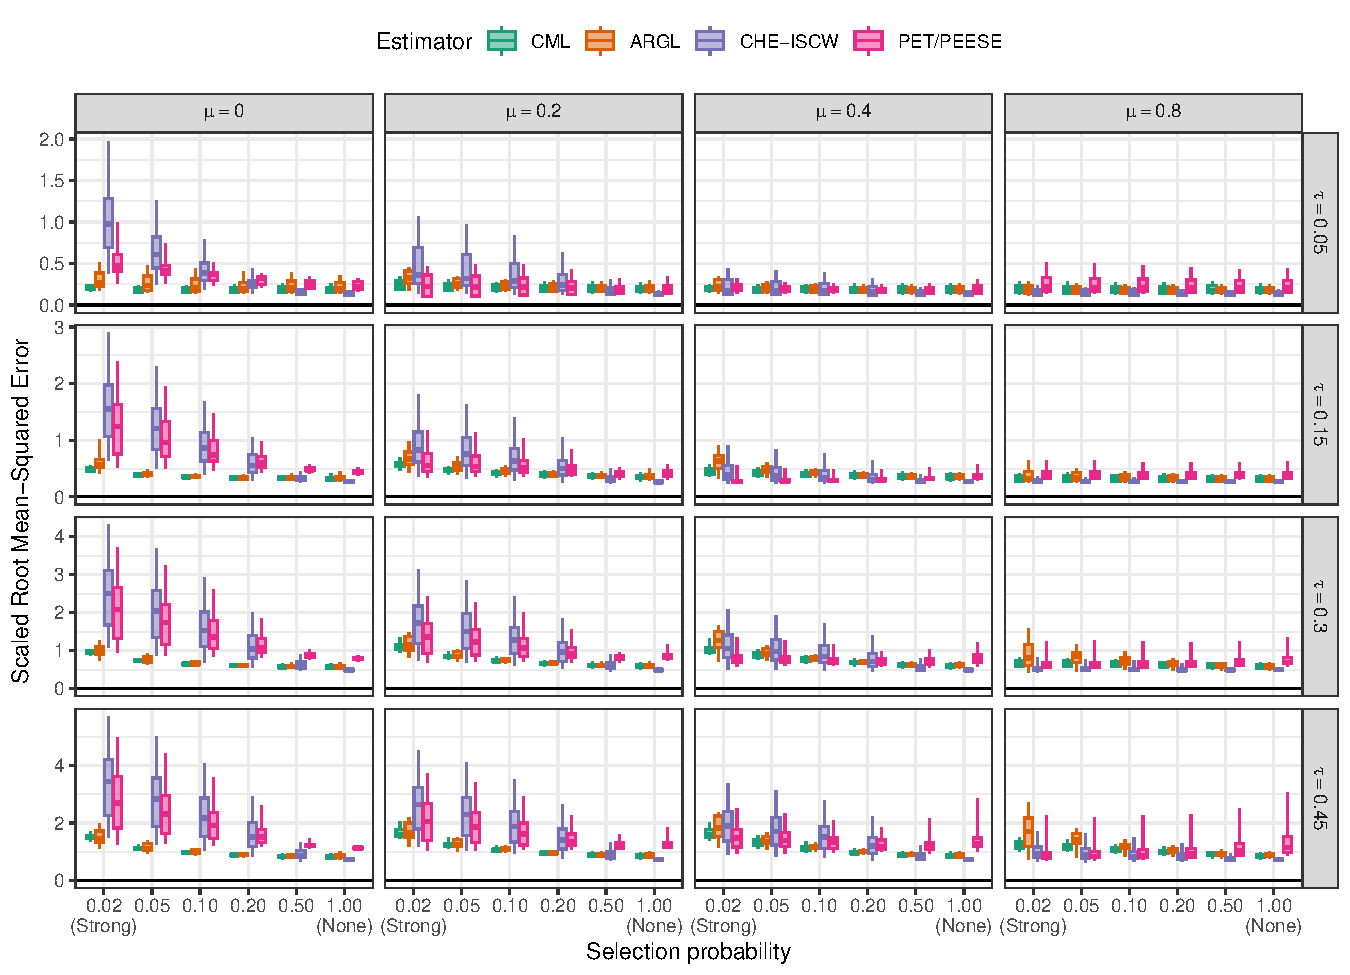
\includegraphics{simulation_results_files/figure-latex/mu-rmse-1} \caption{Scaled root mean-squared error for estimators of average effect size by selection probability, average SMD, and between-study heterogeneity}\label{fig:mu-rmse}
\end{sidewaysfigure}

Scaled RMSE combines both bias and variability into an overall measure
of inaccuracy. Figure @ref(fig:mu-rmse) depicts the scaled RMSE of each
estimator of average effect size; it is constructed in the same way as
Figure @ref(fig:mu-bias). Figures @ref(fig:rmse-ARGL-CML) through
@ref(fig:rmse-PET-ARGL) in Appendix @ref(mu-simulation-results) provide
greater detail about the relative accuracy of the four methods by
plotting the ratio of RMSEs for each pair of methods. These figures
illustrate several findings.

First, across most data-generating conditions, the ARGL estimator has
higher RMSE than the CML estimator. (This is evident in Figure
@ref(fig:rmse-ARGL-CML), which shows that that the RMSE ratio comparing
ARGL to CML is greater than one across most conditions examined.) The
ARGL estimator has lower RMSE only under conditions of very high
heterogeneity and in databases with few studies. Thus, the CML will
typically be preferable to the ARGL estimator.

Second, considering both the selection model estimators and comparison
methods, no single method achieves the lowest RMSE uniformly across all
conditions examined. Instead, all methods face bias-variance trade-offs.
Under conditions with small or moderate average effect size and moderate
or strong selection, the selection model estimators generally have lower
RMSE than the CHE-ISCW and PET/PEESE estimators. The CML estimator has
lower RMSE than CHE-ISCW under most conditions where selective reporting
creates meaningful bias---specifically, for \(\lambda_1 <= 0.2\) and
\(\mu \leq 0.2\) (Figure @ref(fig:rmse-CHE-CML)). The relative accuracy
of the ARGL estimator versus CHE-ISCW follows a similar pattern (Figure
@ref(fig:rmse-CHE-ARGL)).

Third, the CML estimator also has lower RMSE than PET/PEESE under
conditions where selective reporting creates meaningful bias, although
it is not uniformly more accurate than PET/PEESE (Figure
@ref(fig:rmse-PET-CML)). Rather, PET/PEESE is more accurate under
\emph{some} conditions involving moderate or large effect size
\((\mu \geq 0.4)\) and varying degrees of between-study heterogeneity,
which correspond to conditions where the bias of PET/PEESE is small. The
relative accuracy is difficult to characterize generally because it
follows a non-linear pattern involving interactions among the
data-generating parameters. The pattern of relative accuracy is very
similar for the ARGL estimator (Figure @ref(fig:rmse-PET-ARGL)).

The bias-variance trade-offs faced by all the estimators arise because
the CHE-ISCW estimator (which does not directly adjust for selection) is
substantially biased by selective reporting, whereas the CML and ARGL
estimators have at most small biases. However, under conditions where
selection is absent or small and where average effect size is larger,
the CHE-ISCW estimator has greater precision than the estimators that
adjust for selective reporting. Because selective reporting does not
create much bias under such conditions, the additional variability that
comes with estimating a selection model or PET/PEESE adjustment
dominates the small reduction in bias that these methods provide.

\subsubsection{Confidence Interval
Coverage}\label{confidence-interval-coverage}

Figure @ref(fig:comparison-coverage) shows the coverage rates of 95\%
CIs based on large-sample cluster-robust variance estimators for the
CHE-ISCW, PET/PEESE, CML, and ARGL estimators.\footnote{To provide
  greater detail, the vertical axis of Figure
  @ref(fig:comparison-coverage) is limited to the range {[}0.5, 1.0{]},
  and coverage rates of the CHE-ISCW and PET/PEESE intervals are not
  depicted when they fall below 0.5. Supplementary Figure
  @ref(fig:comparison-coverage-full) depicts the full range of coverage
  rates.} Coverage rates are below the nominal rate of 0.95 for all
methods across most conditions. The CML and ARGL estimators based on the
step-function selection model have higher coverage rates than the
comparison methods under many conditions, particularly in conditions
with higher between-study heterogeneity,\\
Intervals based on the CML and ARGL estimators have coverage levels that
improve towards 0.95 as the number of studies increases, but are often
still unacceptably low even when \(J = 90\) or greater. In contrast,
intervals based on CHE-ISCW and PET/PEESE are often wildly
mis-calibrated due to the biases of these estimators. Under conditions
where CHE-ISCW and PET/PEESE are biased by selective reporting, their
confidence intervals do not center on the true parameter. Consequently,
as the number of studies increases, the standard error of the estimators
decreases (as does the width of confidence intervals) and their coverage
rates degrade towards zero.

\begin{Shaded}
\begin{Highlighting}[]
\NormalTok{mu\_graph\_res\_ci }\SpecialCharTok{\%\textgreater{}\%}
  \FunctionTok{filter}\NormalTok{(}
\NormalTok{    CI\_type }\SpecialCharTok{\%in\%} \FunctionTok{c}\NormalTok{(}\StringTok{"large{-}sample"}\NormalTok{)}
\NormalTok{  ) }\SpecialCharTok{\%\textgreater{}\%}
  \FunctionTok{ggplot}\NormalTok{(}\FunctionTok{aes}\NormalTok{(}\AttributeTok{x =}\NormalTok{ J, }\AttributeTok{y =}\NormalTok{ coverage, }\AttributeTok{color =}\NormalTok{ estimator, }\AttributeTok{fill =}\NormalTok{ estimator)) }\SpecialCharTok{+}
  \FunctionTok{geom\_boxplot}\NormalTok{(}\AttributeTok{alpha =}\NormalTok{ .}\DecValTok{5}\NormalTok{, }\AttributeTok{coef =} \ConstantTok{Inf}\NormalTok{) }\SpecialCharTok{+}
  \FunctionTok{geom\_hline}\NormalTok{(}\AttributeTok{yintercept =} \FloatTok{0.95}\NormalTok{, }\AttributeTok{linetype =} \StringTok{"dashed"}\NormalTok{) }\SpecialCharTok{+}
  \FunctionTok{coord\_cartesian}\NormalTok{(}\AttributeTok{ylim =} \FunctionTok{c}\NormalTok{(}\FloatTok{0.5}\NormalTok{, }\FloatTok{1.0}\NormalTok{)) }\SpecialCharTok{+} 
  \FunctionTok{scale\_y\_continuous}\NormalTok{(}\AttributeTok{expand =} \FunctionTok{expansion}\NormalTok{(}\FunctionTok{c}\NormalTok{(}\DecValTok{0}\NormalTok{,}\DecValTok{0}\NormalTok{),}\FunctionTok{c}\NormalTok{(}\FloatTok{0.02}\NormalTok{,}\DecValTok{0}\NormalTok{))) }\SpecialCharTok{+} 
  \FunctionTok{scale\_color\_brewer}\NormalTok{(}\AttributeTok{palette =} \StringTok{"Dark2"}\NormalTok{) }\SpecialCharTok{+}
  \FunctionTok{scale\_fill\_brewer}\NormalTok{(}\AttributeTok{palette =} \StringTok{"Dark2"}\NormalTok{) }\SpecialCharTok{+}
  \FunctionTok{facet\_grid}\NormalTok{(}
\NormalTok{    tau }\SpecialCharTok{\textasciitilde{}}\NormalTok{ mean\_smd, }
    \AttributeTok{labeller =} \FunctionTok{label\_bquote}\NormalTok{(}
      \AttributeTok{rows =}\NormalTok{ tau }\SpecialCharTok{==}\NormalTok{ .(tau),}
      \AttributeTok{cols =}\NormalTok{ mu }\SpecialCharTok{==}\NormalTok{ .(mean\_smd)}
\NormalTok{    ),}
    \AttributeTok{scales =} \StringTok{"free\_y"}
\NormalTok{  ) }\SpecialCharTok{+}
  \FunctionTok{labs}\NormalTok{(}
    \AttributeTok{x =} \StringTok{"Number of studies (J)"}\NormalTok{, }
    \AttributeTok{y =} \StringTok{"Coverage rate"}\NormalTok{, }
    \AttributeTok{color =} \StringTok{"Estimator"}\NormalTok{,}
    \AttributeTok{fill =} \StringTok{"Estimator"}
\NormalTok{  ) }\SpecialCharTok{+} 
  \FunctionTok{theme\_bw}\NormalTok{() }\SpecialCharTok{+}
  \FunctionTok{theme}\NormalTok{(}\AttributeTok{legend.position =} \StringTok{"top"}\NormalTok{)}
\end{Highlighting}
\end{Shaded}

\begin{sidewaysfigure}
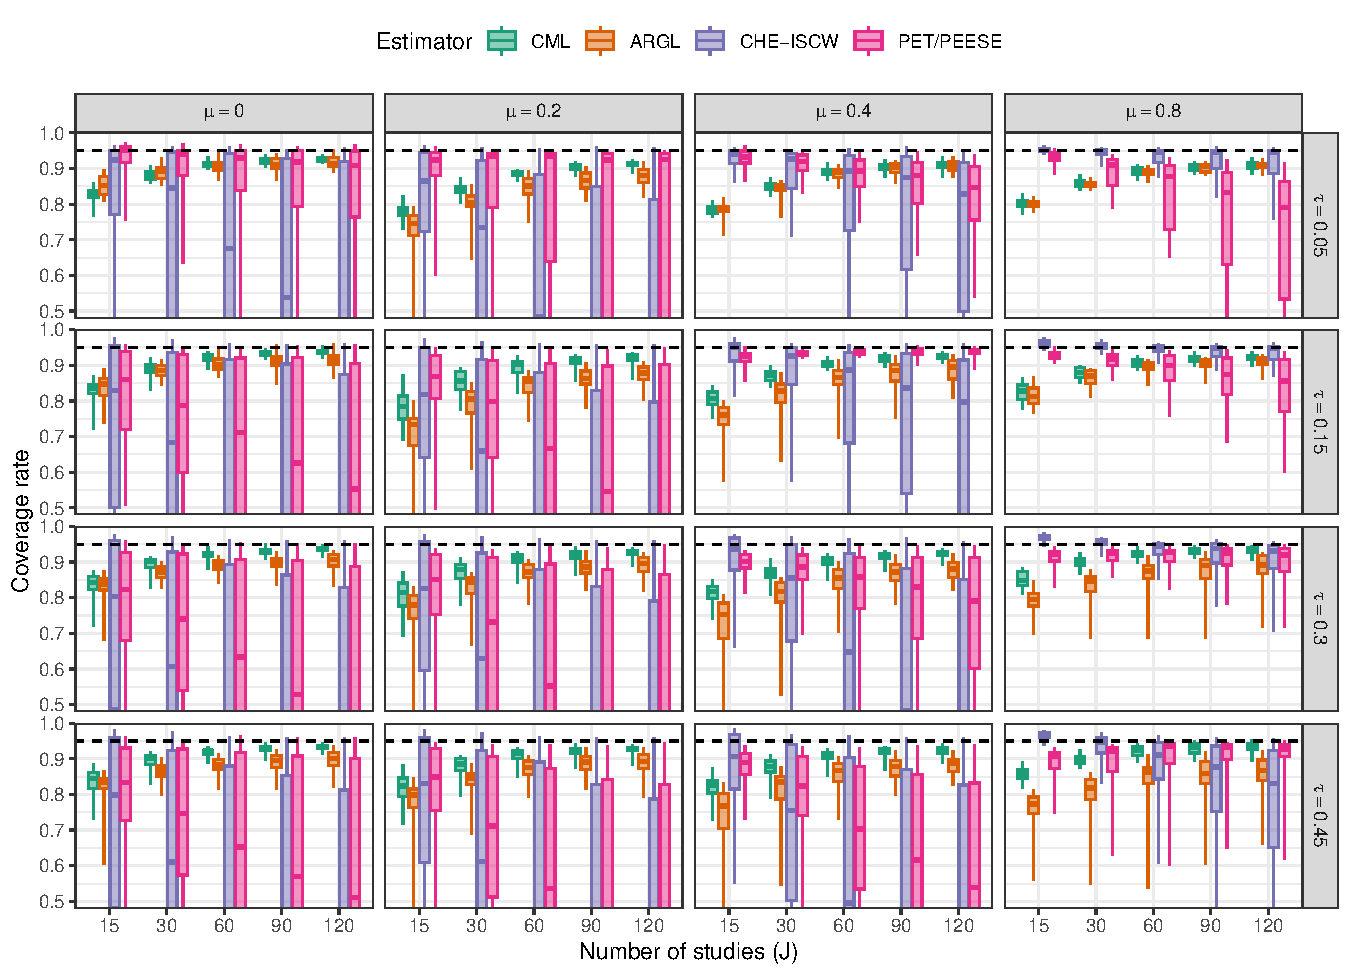
\includegraphics{simulation_results_files/figure-latex/comparison-coverage-1} \caption{Coverage levels of confidence intervals based for average effect size based on cluster-robust variance approximations, by number of studies, average SMD, and between-study heterogeneity. Dashed lines correspond to the nominal confidence level of 0.95. Coverage rates of the CHE-ISCW and PET/PEESE intervals are not depicted when they fall below 0.5}\label{fig:comparison-coverage}
\end{sidewaysfigure}

Bootstrap intervals for the step-function model provide more accurate
coverage levels. Due to the computational demands of bootstrapping, we
evaluated the bootstrap confidence intervals under a more limited range
of data-generating conditions, including a maximum sample size of
\(J = 60\). Figure @ref(fig:CML-coverage) depicts the coverage levels of
confidence intervals based on the CML estimator, including intervals
based on large-sample cluster-robust variance methods and percentile
intervals using either two-stage, multinomial (non-parametric), or
exponential (fractional reweighted) bootstrap resampling. Although none
of the intervals provide exactly nominal coverage, all versions of the
percentile bootstrap intervals have coverage that is closer to nominal
than the intervals based on cluster-robust variance estimation. In
particular, the percentile intervals with two-stage clustered bootstrap
re-sampling provided the best coverage levels, exceeding 90\% coverage
across nearly all data-generating conditions, even with only \(J = 15\)
primary studies per meta-analysis. Coverage levels of the other
bootstrap intervals, including studentized, basic, and BCa intervals,
were not as accurate as percentile intervals (see Supplementary Figures
@ref(fig:CML-coverage-two-stage)-@ref(fig:CML-coverage-exponential) for
detailed results). Coverage levels of intervals based on the ARGL
estimator followed very similar patterns to those for the CML estimator
(Supplementary Figures
@ref(fig:ARGL-coverage-two-stage)-@ref(fig:ARGL-coverage-exponential)).

\begin{Shaded}
\begin{Highlighting}[]
\NormalTok{mu\_graph\_res\_ci }\SpecialCharTok{\%\textgreater{}\%}
  \FunctionTok{filter}\NormalTok{(}
\NormalTok{    bootstrap\_condition }\SpecialCharTok{==} \StringTok{"bootstrap"}\NormalTok{,}
\NormalTok{    estimator }\SpecialCharTok{\%in\%} \FunctionTok{c}\NormalTok{(}\StringTok{"CML"}\NormalTok{),}
\NormalTok{    CI\_type }\SpecialCharTok{\%in\%} \FunctionTok{c}\NormalTok{(}\StringTok{"large{-}sample"}\NormalTok{,}\StringTok{"percentile"}\NormalTok{)}
\NormalTok{  ) }\SpecialCharTok{\%\textgreater{}\%}
  \FunctionTok{ggplot}\NormalTok{(}\FunctionTok{aes}\NormalTok{(}\AttributeTok{x =}\NormalTok{ J, }\AttributeTok{y =}\NormalTok{ coverage, }\AttributeTok{color =}\NormalTok{ CI\_boot\_method, }\AttributeTok{fill =}\NormalTok{ CI\_boot\_method)) }\SpecialCharTok{+}
  \FunctionTok{geom\_boxplot}\NormalTok{(}\AttributeTok{alpha =}\NormalTok{ .}\DecValTok{5}\NormalTok{, }\AttributeTok{coef =} \ConstantTok{Inf}\NormalTok{) }\SpecialCharTok{+}
  \FunctionTok{geom\_hline}\NormalTok{(}\AttributeTok{yintercept =} \FloatTok{0.95}\NormalTok{, }\AttributeTok{linetype =} \StringTok{"dashed"}\NormalTok{) }\SpecialCharTok{+}
  \FunctionTok{scale\_color\_brewer}\NormalTok{(}\AttributeTok{palette =} \StringTok{"Dark2"}\NormalTok{) }\SpecialCharTok{+}
  \FunctionTok{scale\_fill\_brewer}\NormalTok{(}\AttributeTok{palette =} \StringTok{"Dark2"}\NormalTok{) }\SpecialCharTok{+}
  \FunctionTok{facet\_grid}\NormalTok{(}
\NormalTok{    tau }\SpecialCharTok{\textasciitilde{}}\NormalTok{ mean\_smd, }
    \AttributeTok{labeller =} \FunctionTok{label\_bquote}\NormalTok{(}
      \AttributeTok{rows =}\NormalTok{ tau }\SpecialCharTok{==}\NormalTok{ .(tau),}
      \AttributeTok{cols =}\NormalTok{ mu }\SpecialCharTok{==}\NormalTok{ .(mean\_smd)}
\NormalTok{    ),}
    \AttributeTok{scales =} \StringTok{"free\_y"}
\NormalTok{  ) }\SpecialCharTok{+}
  \FunctionTok{labs}\NormalTok{(}
    \AttributeTok{x =} \StringTok{"Number of studies (J)"}\NormalTok{, }
    \AttributeTok{y =} \StringTok{"Coverage rate"}\NormalTok{, }
    \AttributeTok{color =} \StringTok{"Method"}\NormalTok{,}
    \AttributeTok{fill =} \StringTok{"Method"}
\NormalTok{  ) }\SpecialCharTok{+} 
  \FunctionTok{theme\_bw}\NormalTok{() }\SpecialCharTok{+}
  \FunctionTok{theme}\NormalTok{(}\AttributeTok{legend.position =} \StringTok{"top"}\NormalTok{)}
\end{Highlighting}
\end{Shaded}

\begin{sidewaysfigure}
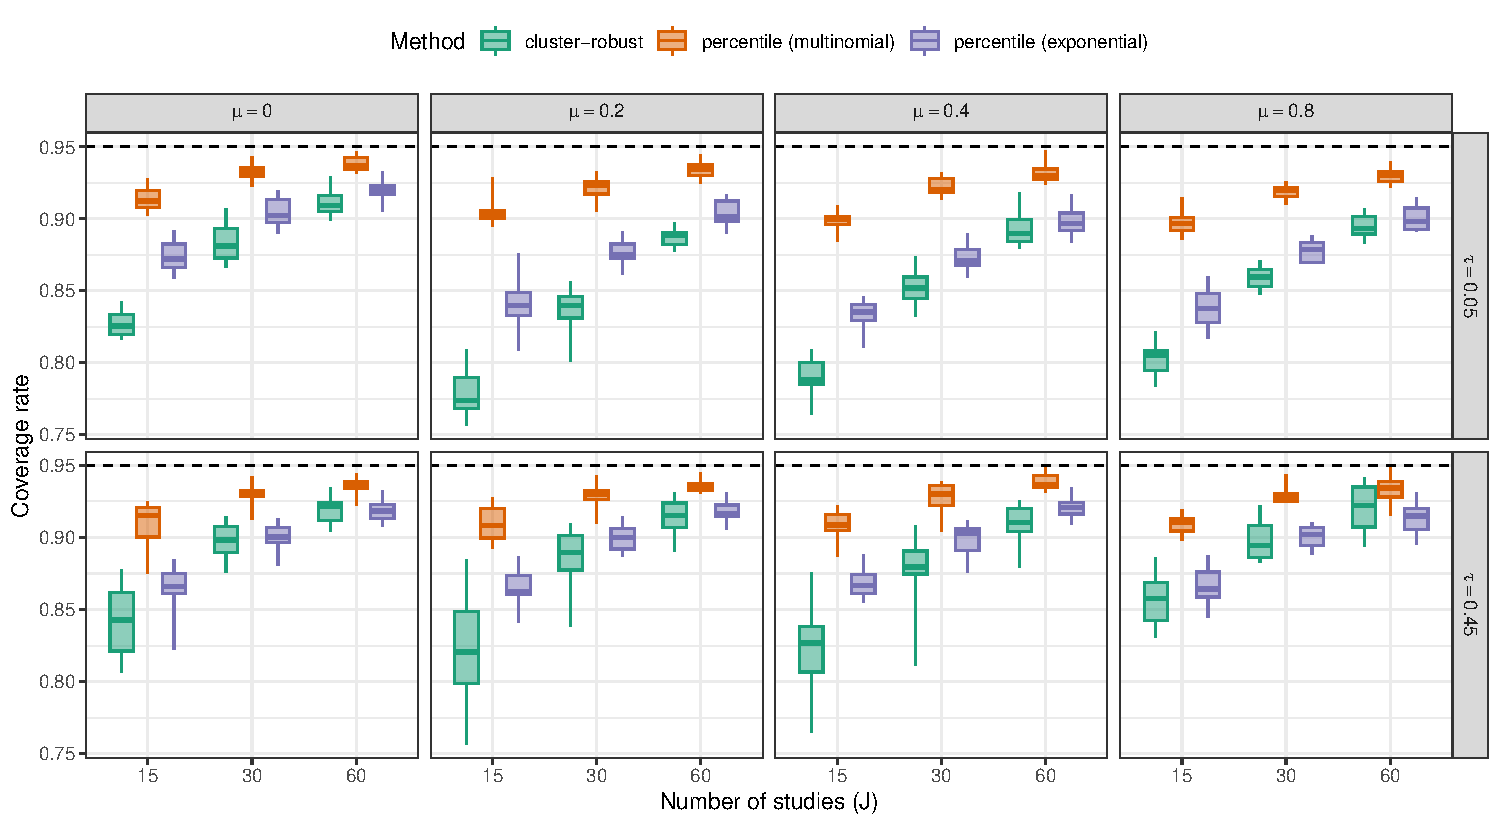
\includegraphics{simulation_results_files/figure-latex/CML-coverage-1} \caption{Coverage levels of confidence intervals based on the CML estimator of average effect size by number of studies, average SMD, and between-study heterogeneity. Dashed lines correspond to the nominal confidence level of 0.95.}\label{fig:CML-coverage}
\end{sidewaysfigure}

\subsection{Effect Size Variance}\label{effect-size-variance}

We briefly consider estimation of the marginal heterogeneity of the
effect size distribution, for which the CHE, CML, and ARGL methods are
all relevant.\footnote{We omitted the variance estimator from the
  CHE-ISCW method because it is identical to that of CHE.} Figure
@ref(fig:heterogeneity-bias) depicts the bias for the CHE, CML, and ARGL
estimators of log-heterogeneity \(\gamma = \log(\tau^2)\). In most
conditions, the estimators are biased in the negative direction. Bias is
high for all three estimators in conditions where the between-study
heterogeneity is low (\(\tau = 0.05\)) with bias improving as
between-study heterogeneity increases. The CML estimator is less
strongly biased than the CHE estimator under conditions where there is
strong selection. However, the ARGL estimator is badly biased downward,
especially under conditions where selection is strong, average SMD is
low and between-study heterogeneity is low.

Figure @ref(fig:heterogeneity-rmse) depicts the scaled RMSE for
estimators of log-heterogeneity, with Figures
@ref(fig:heterogeneity-rmse-ARGL-CHE) and
@ref(fig:heterogeneity-rmse-ARGL-CML) providing greater detail about the
relative accuracy of the three methods. Under nearly all conditions, the
CML estimator is much more accurate than the ARGL estimator. The RMSE of
CML is smaller than that of CHE under some but not all conditions; the
former performs better under conditions where selection is strong,
average SMD is low, between-study heterogeneity is large, and sample
size is large. However, just as with the estimators of average effect
size, the CHE estimator is more accurate when selection is mild or
absent, leading to a bias-variance trade-off.

\subsection{Selection Parameter}\label{selection-parameter}

The CML and ARGL methods both estimate the log-selection parameter of
the step-function model, a parameter that may be of substantive
interest. Figure @ref(fig:selection-bias) shows that the bias of the two
estimators is similar: Both show bias close to zero under conditions
with low average SMD and high between-study heterogeneity but have large
negative biases under conditions with strong selection probability and
high average SMD, especially with low between-study heterogeneity.
Figure @ref(fig:selection-rmse) depicts the RMSE for the ARGL and CML
estimators of the log-selection parameter with Figure
@ref(fig:selection-rmse-ARGL-CML) providing a more detailed view of the
relative accuracy of the ARGL versus the CML estimators. The CML
estimator of the selection parameter generally outperforms the ARGL
estimator, especially under conditions with strong selection. Figures
@ref(fig:CML-zeta-coverage-two-stage) and
@ref(fig:ARGL-zeta-coverage-two-stage) depict the confidence interval
coverage of the two estimators with various bootstrap confidence
interval estimation approaches, using two-stage clustered bootstrap
resampling. Broadly, none of the methods provide coverage rates that are
close to the nominal 95\% level across all conditions examined.

\end{document}
